\documentclass{acm_proc_article-sp}
\usepackage[brazil]{babel}
\usepackage[utf8]{inputenc}
%\usepackage{amsthm}
\usepackage{algorithm}
\usepackage{algpseudocode} % pseudo-código do cormen

\newtheorem{thm}{Teorema}
%opening
\title{Extraindo Nós Influentes para Difusão de Informação em Redes Sociais}
\subtitle{[Trabalho Prático da Disciplina - Projeto e Análise de Algoritmos]}
\numberofauthors{1}
\author{
\alignauthor
  Alcemir Rodrigues Santos \\
  \affaddr{Universidade de Minas Gerais - UFMG}\\
  \affaddr{Instituto de Ciências Exatas - ICEx}\\
  \affaddr{Minas Gerais - Belo Horizonte - Campus Pampulha - CEP 31270-010} \\
  \email{alcemir@dcc.ufmg.br}  
}

\hyphenation{pro-ble-mas}
\begin{document}
\maketitle
\begin{abstract}
% Contexto geral e específico
No mundo atual, com a competitividade entre as empresas que buscam mais espaço no mercado, surgem novas formas de
fazer a propaganda de sua marca. Com o advento das redes sociais, uma delas tomou grande evidência, o
\textit{marketing viral} faz com que a difusão de informação aconteça de forma antes jamais imaginadas. 
% –Questão/problema sendo investigado
Neste artigo trata-se o problema de maximização de influência de nós (indivíduos) de uma rede social para escolha
daquele que tem o maior poder de difundir uma certa informação. %– Propósito do trabalho
%– Estado-da-arte 
As abordagens atuais utilizam métodos de grande complexidade para a aproximação do grau de influência de cada nó, 
%– Por que precisa de uma solução nova/melhor
se por ventura adicionado ao conjunto dos difusores da informação.%– Solução %– Nome da proposta 
Portanto, este trabalho apresenta um método mais simples para a aproximação através de um algoritmo híbrido baseado no paradigma de \textit{força bruta}.
%– Metodologia básica sem detalhes
%– Quais características respondem as questões iniciais
%– Interpretação dos resultados, conclusões

\end{abstract}
% A category with the (minimum) three required fields
\category{F.2}{Análise de algoritmos e complexidade de problemas}{Misto}
%A category including the fourth, optional field follows...
% \category{D.2.8}{Software Engineering}{Metrics}[complexity measures, performance measures]

\terms{Algoritmos, Experimentação, Desempenho}

\keywords{Algoritmos de Aproximação, Marketing Viral, Grau de Influência, Redes Sociais}

\newtheorem{definicao}{Definição}
%===========================================
\section{Introdução}
Com a surgimento das redes sociais na Internet, os usuários conseguiram o espaço que queriam para debaterem sobre diversos assuntos.
Inclusive os que mais os aborreciam, problemas com empresas e/ou produtos e seus atendimentos em \textit{call centers}.
Mas o espaço não estava aberto somente para a reclamação dos usuários, as empresas também apredenram a utilizar-se dela para a sua 
divulgação mais efetiva. 

Falar de uma determinada marca em redes sociais, como o twitter, significa a certeza de ser ouvido por muitas pessoas. Mesmo que elas
não estejam em seu ciclo social. Gerando então o que ficou conhecido como ``Marketing Viral''. Efeito direto da propaganda 
``boca-a-boca'' e que recebe este nome em analogia ao processo de desenvolvimento de uma epidemia viral por uma cidade.

Obviamente, quanto mais influência um usuário tiver frente aos demais, sua mensagem poderá chegar bem mais longe dentro da rede. 
Este é o problema abordado aqui. Como encontrar o conjunto de usuários de maior influência e que proporcionam maior \textit{Difusão
de Informação em Redes Sociais}. Um exemplo prático deste tipo de avaliação pode ser encontrado no sítio web Twitalyzer 
(\textit{www.twitalyzer.com}).

O problema de \textit{seleção do nó mais influente} é NP-difícil \cite{kempe:2003} e pode ser mapeado para o problema de \textit{``Subconjuntos 
independentes máximos''}.

%===========================================
\section{Conceitos Preliminares}
Para este trabalho é considerado um grafo $G = (V,E)$ direcionado. Por direcionado entende-se que as arestas do
conjunto $E$ deste grafo são direcionadas. Ou seja, que dados dois vértices $u$ e $v$ do conjunto $V$, uma aresta
$(u,v)$ só indica o caminho do vértice $u$ para o vértice $v$.

Define-se ainda o conjunto de pais de um vértice $v$, denotado por $\Gamma(v)$ e constituído pelas arestas
que liga um vértice $u$ qualquer, ao, por conseguinte, vértice filho $v$.

O grafo induzido de $G$ é dado por $G' = (V', E')$, onde $V'$ é um subconjunto de $V$ e $E'
= E \cap (V' \times V')$.

Um caminho para o $v_{n}$ partindo do nó $v_{0}$ é escrito da seguinte forma: $(v_{0}, \ldots, v_{n})$, sendo que
$(v_{i-1}, v_{i}) \in E$ com $(i=0,\ldots, n)$. Com isso podemos dizer que o vértice $v_{0}$ pode alcançar o
vértice $v_{n}$, ou ainda, que o vértice $v_{n}$ é alcançável pelo o vértice $v_{0}$. 

Para um vértice $v$ do grafo $G$, define-se $F(v;G)$ como sendo o conjunto de todos os vértices que $v$ pode
alcançar e define-se ainda $B(v;G)$ como sendo o conjunto de todos os vértices que podem alcançar $v$. Para
qualquer $A \subset V$, define-se
$$ 
F(A;G) = \bigcup_{v \in A} F(v;G), B(A;G) = \bigcup_{v \in A} B(v;G).
$$
Um componente fortemente conectado (SCC, do inglês \textit{strongly connected component}) de $G$ é o subconjunto
máximo $C$ de $V$ tal que
$$
\{\forall u,v \in C | \exists (u,\ldots ,v)\}.
$$
Portanto, o $SCC(v;G)$ define o $SCC$ de $G$ que contém $v$. 


%===========================================
\section{Problema da Maximização de Influência}
Kimura \textit{et al.}\cite{kimura:2010} define o modelo matemático de difusão de informação através de uma rede 
social, representada aqui por um grafo $G = (V, E)$. Assumimos para os modelos \textit{Independent Cascade}
(Seção \ref{icm}) e \textit{Linear Threshold} (Seção \ref{ltm}) os seguintes pontos:
\begin{itemize}
  \item Os nós que aceitam a informação são chamados ativos;
  \item O estado de um nó ou é \textit{ativo} ou \textit{inativo};
  \item Os nós podem trocar do estado \textit{inativo} para \textit{ativo}, mas não podem fazer a mudança inversa;
  \item A difusão da informação através da rede \textit{G} é representada pela difusão de nós ativos em
  \textit{G};
  \item Dado um conjunto inicial \textit{A} de nós ativos, supõe-se que os nós em \textit{A} primeiro se tornam
  ativos e os nós restantes continuam inativos no passo $t = 0$.
  \item O processo de difusão de nós ativos acontece em passos discretos de tempo onde $t \geq 0$.
\end{itemize}

\subsection{Modelos Fundamentais de Difusão de Informação}
A representação do problema abordado em redes sociais será dada por um grafo $G = (V,E)$ orientado. Os nós que aceitam a informação 
serão chamados \textit{ativos}. $N$ discrimina o número de nós em $V$ e $L$ o número de arestas em $E$. O conjunto de
nós-pai de um nó $v \in V$ é denominado por $P(v)$.

O processo de difusão ocorre em passos discretos de tempo $t$, onde $t > 0$, e considera-se que um nó sempre iniciará com \textit{status}
\textbf{inativo} e eventualmente mudará para \textbf{ativo}. Não podendo posteriormente retornar ao \textit{status} inativo. Existe um 
conjunto $A$ com os nós ativos. Ao \textit{passo} $0$ o primeiro nó sai do \textit{status} inativo e os demais continuam.

As abordagens para o problema de \textit{Difusão de Informação} encontradas na literatura são basicamente duas e serão utilizadas de
acordo com as definições encontradas em \cite{kempe:2003}. O \textit{Independent Cascade (IC)} e o \textit{Linear Threshold (LT) models} 
serão apresentados em seguida nas subseções \ref{icm} e \ref{ltm}.

  \subsubsection{Modelo de Cascata Independente}\label{icm}
Neste modelo, $p_{u,v}$ é uma constante que representa a probabilidade de propagação através de uma aresta $(u,v)$. Este número 
indica a probabilidade de um nó $u$, quando ativo, ativar cada um de seus nós filhos $v$ em um passo $t$. Isto se dá em chance 
única e caso consiga, o nó filho ativar-se-á no passo subsequente, $t+1$. Um nó $v$ somente se tornará ativo no mesmo passo $t$ quando 
possuir diversos nós-pai que tornaram-se ativos neste mesmo passo. Sendo esta também, a única chance dos nós-pai $u$ ativar o 
nó-filho $v$. É dado fim do processo quando não houver mais ativações possíveis.

Chamamos de ``Grau de Influência'' de um conjunto inicial $A$, o número $\sigma(A)$. Ele representa a quantidade de nós 
ativos no fim do processo.

\begin{thm}
O problema de maximização de influência é NP-Difícil para o modelo de Cascata Independente.
\end{thm}

\begin{proof}
Considere uma instância do problema NP - Completo de \textit{Cobertura de Conjuntos}, definido por uma coleção de
sub-conjuntos $S_{1}, S_{2},\ldots,S_{m}$ de um conjunto universo $U = {u_{1},u_{2},\ldots,u_{n}}$; queremos saber
se existe k dos subconjuntos dos quais a união é igual a $U$. Assumindo que $k < n < m$, mostramos que isto pode
ser visto como um caso especial do problema de maximização de influência.

Dado uma instância do problema de Cobertura de Conjunto, definimos um grafo bipartido direcionado com $n + m$ nós:
existe um nó $i$ correspondente para cada conjunto $S_{i}$, um nó $j$ correspondente a cada elemento $u_{j}$ e uma
aresta $(i,j)$ com probabilidade de ativação $p_{i,j} = 1$ quando quer que $u_{j} \in S_{i}$. O problema de
Cobertura de Conjuntos é equivalente a decidir se existe um conjunto $A$ de $k$ nós no grafo $\sigma(A) \geq
n + k$. Perceba que para a instância definimos que ativação é um processo determinístico, como todas as
probabilidades são $0$ ou $1$. Ativando inicialmente os $k$ nós correspondentes aos conjuntos em uma solução para a
Cobertura de Conjuntos resultando em ativar todos os nós $n$ correspondentes ao universo $U$ e se qualquer conjunto
$A$ de $k$ nós tem $\sigma(A) \geq n + k$, então a Cobertura de Conjuntos deve ser resolvida.
\end{proof}

  \subsubsection{Modelo de Limiar Linear}\label{ltm}
Para cada $v \in V$ neste modelo é necessário especificar um \textit{peso} $w_{u,v} (> 0)$ para os nós-pai $u$ de forma que 
\begin{equation} \label{1}
\sum_{u\in P(v)} w_{u,v} \leq 1 
\end{equation}
Dado um conjunto $A$ e um \textit{limiar} $\theta_{v}$ para cada nó $v$ é escolhido uniformemente ao acaso dentro do intervalo $[0,1]$,
o processo de difusão acontece da seguinte forma:
\begin{enumerate}
  \item Um nó ativo $u$ no passo $t$ influencia o nó $v$ de acordo com $w_{u,v}$;
  \item ($P_{t}(v)$ irá denotar o conjunto de nós-pai de $v$ ativos no passo $t$.)
  \item Se o peso total dos nós-pai ativos é pelo menos o limiar $\theta_{v}$, ou seja, $$\sum_{u\in P(v)} w_{u,v}
  \geq \theta_{v},$$ então $v$ se tornará ativo no passo $t+1$.
\end{enumerate}
Então o processo termina se não houverem mais ativações possíveis.

Chamamos de ``Grau de Influência'' de um conjunto inicial $A$, o número $\sigma(A)$. Ele representa a quantidade de nós 
ativos no fim do processo.

\begin{thm}
O problema de maximização de influência é NP-Difícil para o modelo de Limiar Linear.
\end{thm}

\begin{proof}
Considere uma instância do problema NP - Completo \textit{Cobertura de Vértice} definido por um grafo não
direcionado de $n$ nós $G = (V,E)$ e um inteiro $k$; queremos que se existe um conjunto $S$ de $k$ nós em $G$ então
toda aresta tem pelo menos uma terminação em $S$. Mostramos que isto pode ser visto como um caso especial de
maximização de influência.

Dado uma instância do problema de Cobertura de Vértice envolvendo um grafo $G$, defini-se uma instância
correspondente de maximização de influência direcionando todas as arestas de $G$ em ambas as direções. Se existe uma
cobertura de vértice $S$ de tamanho $k$ em $G$, então ela pode fazer deterministicamente $\sigma(A) = n$ ao
alcançar os nós no conjunto $A = S$; reciprocamente, este é somente o método de encontrar o conjunto $A$ com
$\sigma(A) = n$.
\end{proof}

\subsection{Definição do Problema}
O problema pode ser definido de forma simples, como segue: 

\begin{definicao}
Dado um inteiro positivo $k$, encontre um conjunto $A^{*}_{k} \geq \sigma(B)$ para cada conjunto de $B$ de $k$ nós.
\end{definicao}

Os algoritmos encontrados a literatura pesquisada são geralmente \textit{Algoritmos Gulosos}. Como o algoritmo
de ``Escalada de Montanha'' que foi utilizado em \cite{kimura:2007}. Segue uma breve descrição do algoritmo.

\begin{algorithm}[H]
\caption{Escalada de Montanha}\label{hillclibing}
\begin{algorithmic}[1]
\Procedure{EscaladaDeMotanha}{$G,k$}
	\State $A \gets \varnothing$
	\For{$i\gets 1, k$}
		\State Escolha um nó $v_{i} \in V$ maximizando $\sigma(A \bigcup \{v\})$ \label{estimate_line} \Comment{$(v \in
		V \backslash A)$} \State Faça $A \gets A \bigcup \{v_{i}\}$
	\EndFor
	\State \Return $A$\Comment{O conjunto de nós ativos que maximizam o grau de influência}
\EndProcedure
\end{algorithmic}
\end{algorithm}

\subsubsection{Método Convencional para Estimativa do Grau de Influência}\label{sec-convencional}
Para que a linha \ref{estimate_line} do Algoritmo \ref{hillclibing} seja codificada se faz necessário de um método
para a estimativa do \textit{grau de influência} de cada vértice $v$ que será inserido no conjunto de nós ativos
$A$. Este método foi definido por Kempe \textit{et al.}\cite{kempe:2003} e pode ser visto no Algoritmo .

\begin{algorithm}[H]
\caption{Método Convencional para Estimativa do Grau de Influência}\label{convencional}
\begin{algorithmic}[1]
\Procedure{MetodoConvencional}{}
	\For{$m\gets 1, M$}
		\State Calcule $\varphi(A \cup \{v\})$. 		
		\State Faça $x_{m} \gets \varphi(A \cup \{v\})$.
	\EndFor
	\State Faça $\sigma(A \cup \{v\}) \gets (1/M)\sum^{M}_{m=1} x_{m}$.
\EndProcedure
\end{algorithmic}
\end{algorithm}

Onde, cada $\varphi(A \cup \{v\})$ é computado assim:

\begin{algorithm}[H]
\caption{}\label{}
\begin{algorithmic}[1]
\Procedure{}{}
	\State Faça $H_{0} \gets A \cup \{v\}$.
	\State Faça $t \gets 0$.
	\While{$H_{t} \not= \varnothing $}
		\State Faça $H_{t+1} \gets \{\textnormal{nós ativados no passo} t+1\}$.
		\State Faça $t \gets t+1$.
	\EndWhile
	\State Faça $\varphi(A \cup \{v\}) \gets \sum^{t-1}_{j=0} |H_{j}|$
\EndProcedure
\end{algorithmic}
\end{algorithm}

%===========================================
\section{Estado-da-Arte}
No trabalho de Kimura \textit{et al.} tomado como referência foi apresentado um método alternativo ao mostrado na
seção \ref{sec-convencional}. Utilizaram para a elaboração do método a \textit{bond percolation}, a teoria dos grafos. A partir da análise da complexidade computacional do método e a
posterior comparação mostrou-se mais eficiente que o Algoritmo \ref{convencional}.Segue o algoritmo proposto por
Kimura \textit{et al.} \cite{kimura:2007} e posteriormente melhor fundamentado \cite{kimura:2010}.

\begin{algorithm}[H]
\caption{Método Proposto por Kimura \textit{et al.}}\label{kimura}
\begin{algorithmic}[1]
\Procedure{}{}
	\State Encontre o subconjunto $F(A;G_{r})$ de $V$.
	\State Faça $|F(A \cup \{v\};G_{r})| \gets |F(A;G_{r})|$ para todo $v \in F(A;G_{r}) \backslash A$.
	\State Encontre o subconjunto $V_{r}^{A} = V \backslash F(A;G_{r})$ of $V$, e o grafo induzido $G_{r}^{A}$ de $G_{r}$ a
	$V_{r}^{A}$.
	\State Faça $U \gets \varnothing$.
	\While{$V_{t}^{A} \backslash U \not= \varnothing $}
		\State Pegue o vértice $u \in V_{r}^{A} \backslash U$.
		\State Encontre o subconjunto $F(u;G_{r}^{A})$ de $V_{r}^{A}$.
		\State Encontre o subconjunto $C(u;G_{r}^{A}) = B(u;G_{r}^{A}) \cap F(u;G_{r}^{A})$ de $F(u;G_{r}^{A})$.
		\State Faça $|F(A\cup{v};G_{r}| \gets |F(u;G_{r}^{A})| + |F(A;G_{r}^{A})|$ para todos $v \in C(u;G_{r}^{A})$.
		\State Faça $U \gets U \cup C(u;G_{r}^{A})$.
	\EndWhile
\EndProcedure
\end{algorithmic}
\end{algorithm}

\subsection{Dificuldades encontradas na implementação}
Ao término da leitura do trabalho de referência \cite{kimura:2007}, chegou-se a conclusão de inviabilidade de
implementação do método apresentado por eles. O algoritmo que é apresentado apenas significa uma parte para a
solução do problema, não sendo suficiente para o completo entendimento do mesmo apenas com a da descrição do
algoritmo descrito no trabalho.

Após pesquisa sobre o problema, não foram encontradas boas referências, o trabalho de Kempe\cite{kempe:2003} foi o
que mais se aproximou do trabalho de referência. Até encontrar um trabalho do mesmo grupo de Kimura que extendia o
trabalho inicial publicado somente 3 anos após o primeiro \cite{kimura:2010}.

Com muito esforço e ajuda do segundo trabalho de Kimura \textit{et al.} começou-se a entender o problema mais
claramente e a trabalhar em sua implementação. 

%===========================================
\section{Método Proposto}
O método posposto por este trabalho é baseado no paradigma de projeto de algoritmos denominado \textit{força
bruta} e foi elaborado baseado no método convencional. Para a aproximação do grau de influência exercido
por cada indivíduo (denominado \textit{difusor da informação}) na rede social é feita a contabilização de quantas 
instâncias de indivíduos conectados à esta rede (denominados \textit{nós-alvo}) o difusor consegue alcançar. 

Para isto é feito o caminhamento por toda as árvore geradora do grafo que representa as conexões da rede social
pelas quais houve de fato a propagação da informação, partindo do indivíduo difusor da informação até chegar-se ao
fim das possibilidades de caminhamento. O caminhamento pela árvore é feito por meio de uma busca em largura na
lista de adjacência de cada nó avaliado num dado instante.

\begin{algorithm}[H]
\caption{Método Proposto para Estimativa do Grau de Influência}\label{metodoproposto}
\begin{algorithmic}[1]
\Procedure{MetodoProposto}{}
	\For{$m\gets 1, M$}
		\State Calcule $|F(A \cup \{v\});G_{r}|$, $\forall v \in V \backslash A$.
		\State Calcule $|F(A);G_{r}|$, $\forall v \in A$ 		
		\State Faça $x_{v,m} \gets |F(A \cup \{v\};G_{r})|$,  $\forall v \in V \backslash A$.
		\State Faça $x_{v,m} \gets |F(A);G_{r}|$,  $\forall v \in A$. 
	\EndFor
	\State Faça $\sigma(A \cup \{v\}) \gets (1/M)\sum^{M}_{m=1} x_{m}$.
\EndProcedure
\end{algorithmic}
\end{algorithm}

Os nós ativos da rede, ou seja, os nós que iram iniciar a difusão da informação, recebem um tratamento especial.
Isto pode ser percebido no algoritmo \ref{metodoproposto}. Isto é proposto pois eles fazem parte do conjunto que
maximiza o alcance dentro do grafo e para eles é atribuído o maior valor encontrado para todos os elementos do grupo.

Assim fica descrito o algoritmo proposto para a estimativa do grau de influência de um nó dentro das arestas
``ocupadas'' do grafo.

\subsection{Aspectos técnicos}
Ambas as implementações foram feitas com a linguagem JavaSE versão 1.6 e exutadas sobre a máquina vitual Java
fornecida pela \textit{Oracle}\footnote{http://www.oracle.com}. Foi parcialmente testada com o auxílio de ferramentas como
JUnit\footnote{http://www.junit.org} versão 4 e do hamcrest\footnote{http://code.google.com/p/hamcrest}, que ajudou
nas asserssões. Utilizou-se a IDE Eclipse versão 3.6 (Helios) release 2 e a técnica de \textit{Test Driven
Development} com para condução do desenvolvimento.

Mais detalhes sobre a configuração do ambiente utilizado na seção de Experimentos (\ref{experimentos}).

%=========================================== 
\section{Experimentos}\label{experimentos}
Os experimentos foram todos conduzidos no ambiente restrito de um computador portátil pessoal de configuração
razoável, como segue:

\begin{itemize}
  \item CPU Intel Pentium Dual Core T2130 de $1.86 Hz$;
  \item Memória RAM de aproximadamente $2 GB$; 
  \item Disco Rígido de aproximadamente $120 GB$.
\end{itemize}

O compudador opera com sistema operacional de distribuição livre, Ubuntu\footnote{http://www.ubuntu.com} versão
10.10, com kernel 2.6.35.28-generic e gerenciador de janelas GNOME 2.32.0. 

Os dados referentes ao tempo de execução consideram apenas a execução dos algoritmos para estimar o grau de
influência de um nó do grafo. E foram auferidas com o método simples (\textit{System.currentTimeMillis();})
da API da linguagem Java ao início, ao final da execução e em seguida feita a subtração dos dois valores. Gráficos
do uso de CPU e de memória Heap foram gerados pela ferramenta de monitoramento de aplicações Java chamada
VisualVM\footnote{http://visualvm.java.net/}

Em cada uma das sub-seções seguintes, são apresentados os dados coletados após a execução dos algoritmos na
máquina descrita acima. No momento da execução dos algoritmos, nenhuma outra aplicação era executada em primeiro
plano. Isto foi feito para proporcionar que aos algoritmos uma rápida resposta da máquina utilizada quando da
requisição de mais recursos.

Em seguida são exibidos os dados coletados com os experimentos.

%===========================================
\subsection{Resultados}
Nesta seção são apresentados os dados do experimento realizado com os dois algoritmos tratados neste trabalho, o
algoritmo de Kempe \textit{et al}. e o método proposto por este trabalho.

Os experimentos foram conduzidos inicialmente utilizando o número de iterações \textit{M}, definida no algoritmo
\ref{convencional}, igual a 1000. O experimento consistiu em executar os algoritmos apresentados por \textit{M}
iterações para ao final calcular a média dos números de nós do conjunto final de nós ativados pelo processo de
difusão. Este processo foi reexecutado para pequenos e médios conjuntos de nós ativados de tamanhos iguais a 25,
50, 100, 200, e 500.

O conjunto do nós ativos bem como as arestas do grafo, as quais representavam a difusão da informação, foram 
gerados aleatoriamente e adicionados a um arquivo texto. O arquivo é lido, monta-se o grafo e em seguida começa-se
o processo de estimativa.

\subsubsection{Sobre o Tempo de execução}
No Gráfico \ref{runtime} é mostrado o relacionamento do número de nós ativados pelo processo de difusão em relação
ao tempo de execução em segundos. Note que para fins de melhor apresentação foi aplicado a função logaritmo
utilizando a base 10 ao valor contabilizado para o tempo de execução como aponta o gráfico. Os dados utilizados
para a construção do Gráfico \ref{runtime} são apresentados na Tabela \ref{tabtempo}.

\begin{figure}[ht]%[h|t|b|p]
\centering
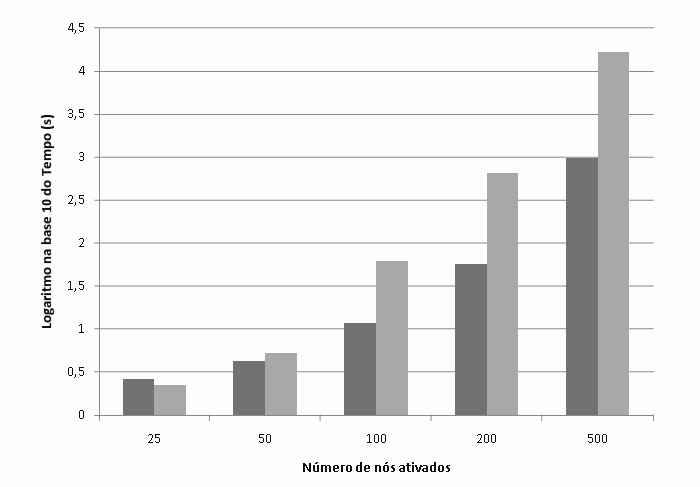
\includegraphics[scale=.35]{img/nosXtempo.png}
\caption{Relacionamento do \textit{Número de nós ativados} versus \textit{$log_{10}$(Tempo de execução em
segundos)}.}
\label{runtime}
\end{figure}

Inicialmente o método teve um desempenho melhor que o método de Kimura \textit{et al.}. Contudo, perceba que o
método proposto não teve um bom desempenho com grafos de tamanhos maiores. 

\begin{table}[!h] \label{tabtempo}
\centering
\begin{tabular}{|c|c|c|}
\hline 
\hline \textbf{no. de nós}  & \textbf{Proposto (s)} & \textbf{Literatura (s)}\\
\hline 
\hline \textbf{$25$}   & $2,214$  & $2,654$\\
\hline \textbf{$50$}   & $5,216$  & $4,262$\\
\hline \textbf{$100$}  & $62,051$ & $11,815$\\
\hline \textbf{$200$}  & $649,582$ & $57,099$\\
\hline \textbf{$500$}  & $16442,073$ & $962,940$\\
\hline \hline
\end{tabular}
\caption{Tempo de execução dos dois algoritmos dado em milisegundos.}
\end{table}

O Gráfico \ref{runtime} mostra claramente o comportamento não polinomial do problema. Com o aumento da quantidade
de nós a serem analisados, aumenta de forma semelhante à uma curva exponencial. 

\subsubsection{Consumo geral de CPU}
As Figuras  \ref{cpu-usage} e \ref{heap-usage} mostram o uso da CPU e da Heap durante a execução dos algoritmos com
o grafo de 200 nós. As grandes oscilações percebidas nos gráficos em instantes próximos ao metade da execução
correspondem exatamente ao instante em que encerra-se a execução do algoritmo de referência e passar-se-ia então à
execução do algoritmo proposto.

\begin{figure}[ht]%[h|t|b|p]
\centering
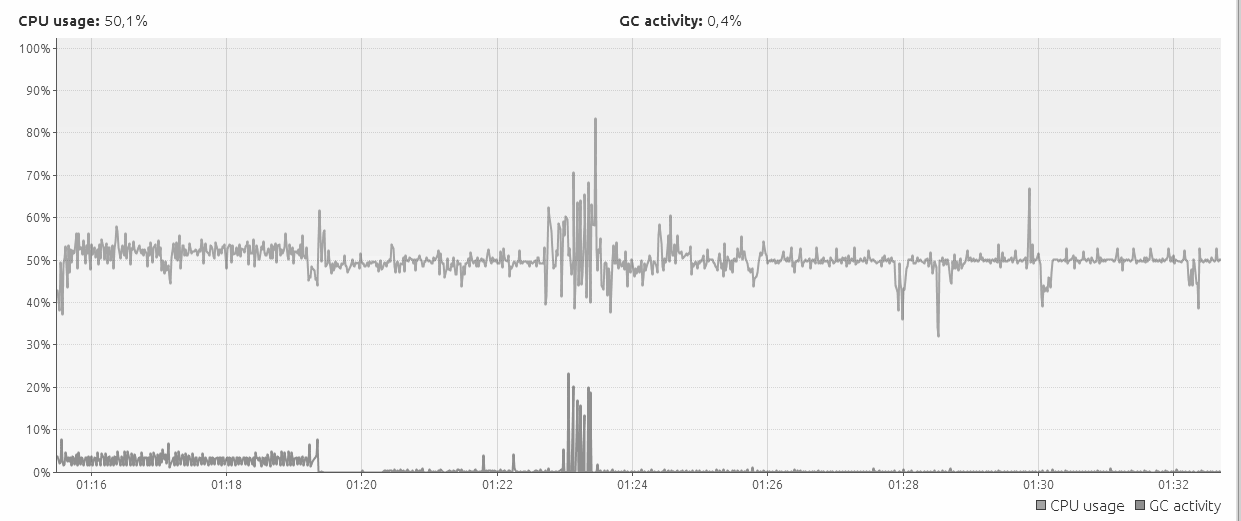
\includegraphics[scale=.2]{img/CPU_usage-200_1000.png}
\caption{Uso da \textit{CPU} durante o processamento do grafo de 200 nós.}
\label{cpu-usage}
\end{figure}

\begin{figure}[ht]%[h|t|b|p]
\centering
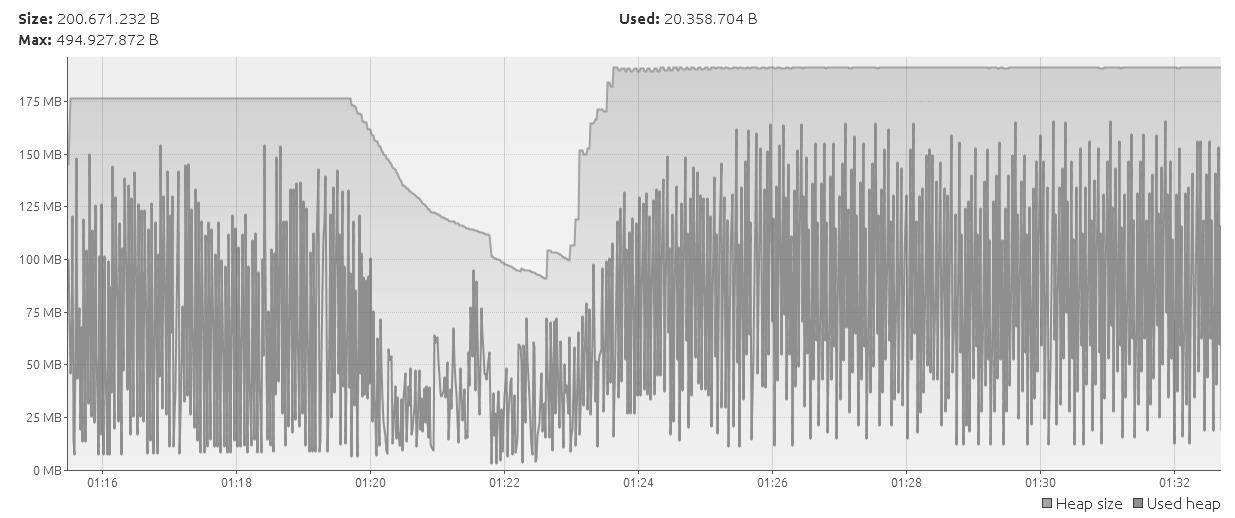
\includegraphics[scale=.2]{img/MemoryHeap_Usage-200_1000.png}
\caption{Uso da \textit{Heap} durante o processamento do grafo de 200 nós.}
\label{heap-usage}
\end{figure}

%===========================================
\section{Análise}

Nesta seção serão apresentados alguns gráficos e dados produzidos para fins de uma análise estatística.
 
%TODO Inserir gráficos com comparativos;
\begin{figure}[ht]%[h|t|b|p]
\centering
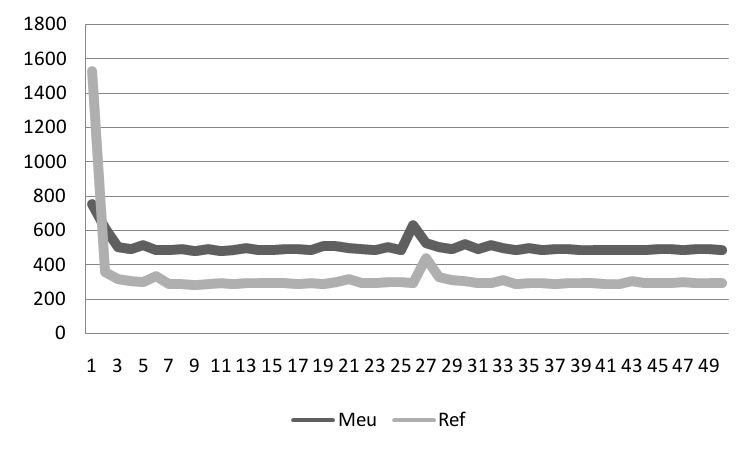
\includegraphics[scale=.3]{img/25nos.png}
\caption{Variação do tempo em 50 iterações de execução com 25 nós.}
\label{25nos}
\end{figure}

\begin{figure}[ht]%[h|t|b|p]
\centering
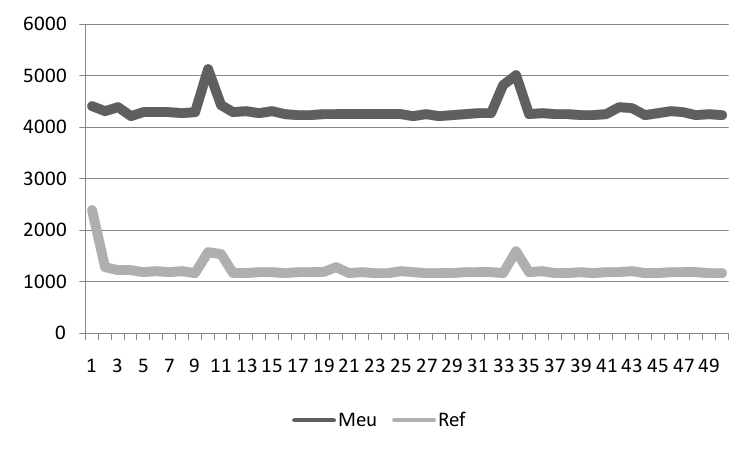
\includegraphics[scale=.3]{img/50nos.png}
\caption{Variação do tempo em 50 iterações de execução com 50 nós.}
\label{50nos}
\end{figure}

\begin{figure}[ht]%[h|t|b|p]
\centering
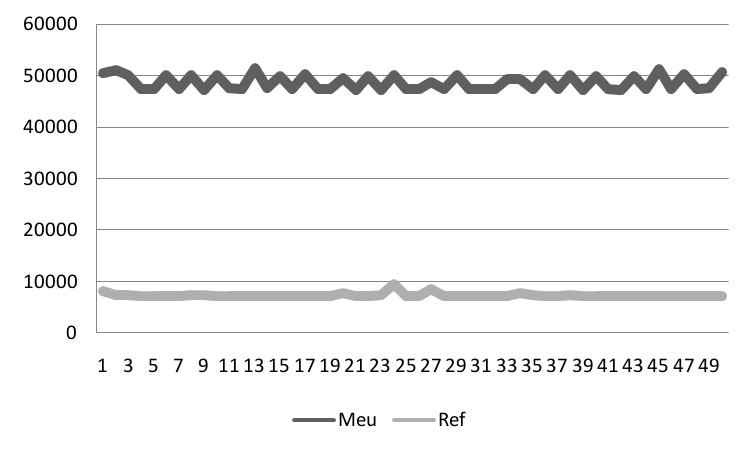
\includegraphics[scale=.3]{img/100nos.png}
\caption{Variação do tempo em 50 iterações de execução com 100 nós.}
\label{100nos}
\end{figure}

Os gráficos \ref{25nos}, \ref{50nos} e \ref{100nos} mostram variação do tempo em 50 iterações de execução
com 25, 50 e 100 nós, respectivamente. A curva de cor mais escura representa o tempo de execução do método
proposto e a mais clara o tempo de execução do método de Kimura \textit{et. al.}. É perceptível que a medida que
aumenta a quantidade de nós a distância entre os tempos de execução também aumenta.

%TODO Inserir tabela com comparativos;
Para uma análise mais apurada, os algoritmos foram submetidos a execuções repetidas com quantidades de nós
diferentes. Coletou-se os dados e em seguida faremos análise dos dados baseada nos resultados da aplicação do Teste
T-pareado. Foram executadas 50 repetições de cada execuções e auferidos os tempos de cada uma delas.

\begin{table}[!h] \label{tabpareado}
\centering
\begin{tabular}{|c|c|c|c|}
\hline 
\hline\textbf{no. de nós}  & \textbf{T.M.(s)} & \textbf{D.P.(s)} &\textbf{I.C.(95\%) }\\
\hline 
\hline \textbf{$25$}   & $181,28$  & $141,04$ & $(167,83; 194,73)$\\
\hline \textbf{$50$}   & $3080,74$  & $196,27$ & $(3062,02; 3099,46)$\\
\hline \textbf{$100$}  & $41418,8$ & $1413,93$ & $(41283,93; 41553,67)$\\
\hline \hline
\end{tabular}
\caption{Resultado da aplicação do Teste T pareado.}
\end{table}

A Tabela \ref{tabpareado} possui os dados da aplicação do Teste T-pareado. A tabela é composta por 4 colunas, cada
uma delas indica o número de nós existentes no grafo, a média das diferenças entre os tempos de execução dos
algoritmos medido em segundos, o desvio padrão também medido em segundos e o intervalo de confiança com 95\% de
confiança, respectivamente. Este teste evidenciou a melhor eficiência do algoritmo tomado como referência.

%===========================================
\section{Conclusão}
A análise estatística feita para a comparação dos algoritmos deste experimento, mostrou que o método proposto
falhou em melhorar o desempenho algoritmo utilizado para comparação sendo encontrado na literatura. Após análise
mais íntima entre os dois métodos, o método proposto perde muito e torna-se muito ingênuo frente ao método proposto
por Kimura \textit{et al.} ao ignorar a ideia de componentes fortemente conectados.

Frente aos resultados expostos neste estudo é possível concluir que o trabalho de Kimura \textit{et al.} tem
desempenho superior ao método proposto. O fato do  método de Kimura \textit{et al.} utiliza-se do conceito de
\textit{componentes fortemente conectados} implica na redução do custo computacional do seu algoritmo para ao
tempo da estimativa do grau de influência de cada nó que não pertence ao conjunto dos nós ativos.


%===========================================
\bibliographystyle{abbrv}
\bibliography{document} 

\end{document}